\subsection{Grundlagen der Optimierung}
Bei der Optimierung betrachtet man vor allem Funktionen, welche Elemente eines $n$-dimensionalen Vektorraumes auf reelle Zahlen abbilden:

\begin{equation*}
f: \mathbb{R}^n \rightarrow \mathbb{R}
\end{equation*}

Beispielhafte Anwendungszwecke wären die Minimierung oder Maximierung der Kosten bzw. der Einnahmen eines Unternehmens. Diese würden dem reellen Funktionswert der Funktion entsprechen und ergäben sich aus den Eigenschaften des Unternehmens wie Gehalt, Anzahl der Mitarbeiter, Marketing-Ausgaben usw., welche man zusammenfassend als Vektor eines $n$-dimensionalen Vektorraumes darstellen könnte.

\subsection{Regression}

\begin{Thm}[Methode der kleinsten Quadrate]
Beispiel für die Lösung eines solchen Minimierungsproblems wäre die Methode der kleinsten Quadrate. Gegeben ist hierbei eine lineare Funktion $f$ und Punkte $P_i=(x_i,y_i)$, welche näherungsweise auf der Geraden liegen:

\begin{align*}
f(x) &= ax \\
y_i &= f(x_i) + \epsilon_{i}
\end{align*}

\begin{dsafigure}
\begin{center}
\includegraphics[width=0.5\textwidth]{\media Grafik-OptimierungLennart_LineareRegression.pdf}
\caption{Konvexe Funktion}
\label{figure:Grafik-OptimierungLennart_LineareRegression.pdf}
\end{center}
\end{dsafigure}

Wenn nun der Abstand $\epsilon_i$ minimiert werden soll, dann gilt:

\begin{equation*}
\min h(x)=\frac{\sum_{i=1}^n(y_i-ax_i)^2)}{e(y_i,x_i)}
\end{equation*}

Hierbei könnte $e^2,\mid e\mid, h(e)$ exemplarische Möglichkeiten seien. Zur Berechnung dieses Minimums gibt es nun verschiedene Möglichkeiten:

\begin{enumerate}
\item Gewöhnliche Tiefpunktberechnung \\
z.~B.$\qquad h'(a)=0\qquad \wedge\qquad h''(a)>0$
\item Gradientenabstiegsmethode \\
$a^{t+1}  =a^{t} - \lambda \cdot \delta f(a^{t})$ \\
Man findet also ein $\lambda > 0$, sodass
$f(a^{t+1}) < f(a^{t})  \qquad \mid \delta f(a^{(t)}) \neq 0$ \\
$g^{+}(\lambda)=f(a^+-\lambda\Delta f(a^t))$ \\
$\lambda^+=argmin(g^+(\lambda))$
\end{enumerate}

\end{Thm}

\begin{Def}[Lokales und globales Minimum]
Für $f: D\rightarrow \mathbb{R}$ ist $x\in D$ ein lokales Minimum, wenn mindestens eine Umgebung $N$ existiert, sodass \\$\forall_{y\in N}$ gilt: $f(y)>=f(x)$ \\
$x\in D$ ist dann ein globales Minimum, falls $N=D$.
\end{Def}

\subsection{Konvexität}
%\begin{Def}[Konvexe Funktion]
%Eine Funktion $f: \mathbb{R}^n\rightarrow\mathbb{R}$ ist dann eine konvexe Funktion, falls $\forall_{x,y\in D}$ gilt: 
%\[f(\lambda x+(1-\lambda)y)\leq\lambdaf(x)+(a-\lambda)f(y)\qquad\mid \forall_{y\in[0,1]}\]
%$\begin{figure}[htbp] 
%  \centering
%     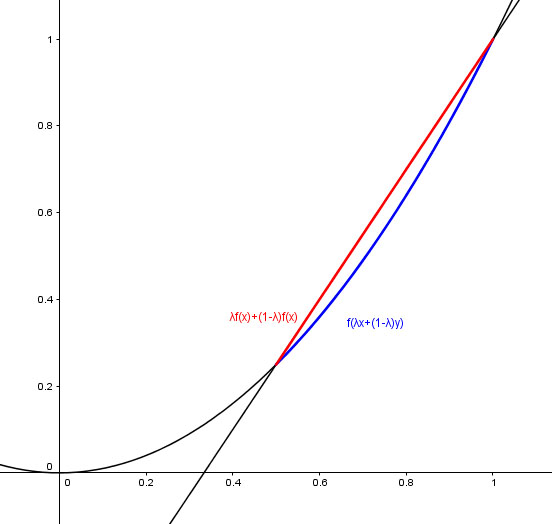
\includegraphics[width=0.7\textwidth]{konvexe_funktion.jpg}
%  \caption{konvexe Funktion}
%  \label{fig:Konvexe Funktion}
%\end{figure}
%	\subsubsection{Beispiel zur Konvexität}
%	\[f(u)=\mid\mid u\mid\mid_2^2\qquad\mid u\in\mathbb{R}\]
%	\[f(\lambda u+(1-\lambda)v)=\mid\mid\lambda u+(1-\lambda)v\mid\mid_2\]
%	\[\leq\mid\mid\lambda u\mid\mid_2+\mid\mid(1-\lambda)v\mid\mid_2\]
%	\[\leq\lambda\mid\mid u\mid\mid_2+(1-\lambda)\mid\mid v\mid\mid_2\]
